\documentclass[conference]{IEEEtran}
\usepackage{graphicx}
\usepackage{amsmath,amsthm,amssymb}
\usepackage{listings}
\usepackage{caption}
\usepackage{cite}
\usepackage{listings}
\usepackage{xcolor}

\lstdefinestyle{cppstyle}{
  language=C++,
  basicstyle=\ttfamily\small,
  keywordstyle=\color{blue}\bfseries,
  commentstyle=\color{gray},
  stringstyle=\color{orange},
  numbers=left,
  numberstyle=\tiny\color{gray},
  stepnumber=1,
  numbersep=8pt,
  frame=single,
  breaklines=true,
  tabsize=2,
  showstringspaces=false,
  captionpos=b
}

\usepackage{comment}





\title{Greedy and Divide-and-Conquer Algorithms: \\ Interval Scheduling and Closest Pair}
\author{\IEEEauthorblockN{Your Name(s)}
\IEEEauthorblockA{Department \\ University \\ email@university.edu}}
\begin{document}
\maketitle
\begin{abstract}
Two canonical algorithmic techniques are demonstrated on practical problems: a greedy solution for appointment scheduling, and a divide-and-conquer solution for the closest pair of points. Each problem includes abstraction, algorithm, analysis, correctness sketch, domain explanation, and experimental verification.
\end{abstract}

\section{Introduction}
We present two problems and their solutions: clinic appointment scheduling (solved optimally by a greedy policy) and the geometric closest-pair (solved with divide-and-conquer).

\section{Greedy: Clinic Appointment Scheduling}

\subsection{Domain}
\textbf{Problem:} Maximize the number of patient appointments accepted in a single clinic room in a day.  

\textbf{Motivation:} Clinics must schedule appointments of varying lengths and start windows. With a single resource (one room or one physician), we aim to accept as many non-overlapping appointments as possible. This is a real operational problem relevant to hospital outpatient management and home-health scheduling.  

\subsection{Abstraction}
We model the problem as the classical \emph{interval scheduling problem}:  

Let 
\[
I = \{1,2,\dots,n\}
\]
be the set of appointment requests.  

Each request $i$ has a start time $s_i$ and finish time $f_i$, with $s_i < f_i$.  

Two requests $i,j$ are compatible if their intervals do not overlap:
\[
f_i \le s_j \quad \text{or} \quad f_j \le s_i.
\]

\textbf{Goal:} Find a maximum-cardinality subset $S \subseteq I$ of pairwise-compatible requests.  

This is a set/interval abstraction (sets of time intervals).  

\subsection{Algorithm  — Greedy: Earliest-Finish-Time-First (EFTF)}
\textbf{Pseudocode:}
\begin{verbatim}
Input: list of intervals (s_i, f_i) 
for i = 1..n
Sort intervals by finish time f_i nondecreasing.
A = empty list
last_finish = -infty
for (s,f) in sorted_intervals:
    if s >= last_finish:
        append (s,f) to A
        last_finish = f
return A
\end{verbatim}

\subsection{Running Time Analysis}
\begin{itemize}
    \item Sorting intervals by finish time: $O(n \log n)$
    \item Single scan to select compatible intervals: $O(n)$
    \item Total: $T(n) = O(n \log n)$
\end{itemize}

\subsection{Proof of Correctness}

We prove that the greedy algorithm produces an optimal set of jobs.  

Let the greedy solution be 
\[
G = \{i_1, i_2, \dots, i_k\},
\]
and let an optimal solution be 
\[
O = \{j_1, j_2, \dots, j_m\}.
\]

\textbf{Step 1: Proof setup (by contradiction)}  

Assume $G$ is not optimal, i.e., $|G| < |O|$.  

Let $i_1, i_2, \dots, i_k$ be the jobs selected by the greedy algorithm, and $j_1, j_2, \dots, j_m$ be jobs in the optimal solution.  

Define $r$ to be the largest index such that
\[
i_1 = j_1, \ i_2 = j_2, \ \dots, \ i_r = j_r
\]
i.e., the first $r$ jobs of both solutions match.  

\textbf{Step 2: Critical observation}  

By the greedy choice rule, the next job $i_{r+1}$ selected by the greedy algorithm finishes as early as possible among all compatible jobs. That is,
\[
f(i_{r+1}) \le f(j_{r+1}).
\]  

\textbf{Step 3: Replacement argument}  

Replace $j_{r+1}$ in $O$ with $i_{r+1}$. The new solution remains feasible because $i_{r+1}$ finishes no later than $j_{r+1}$ and does not overlap with the remaining jobs in $O$.  

Thus, the new optimal solution now matches $G$ for one more position (up to $r+1$).  

\textbf{Step 4: Contradiction}  

This contradicts the assumption that $r$ was the largest index where $G$ and $O$ agreed. Hence, our assumption that $G$ is not optimal is false.  

\textbf{Conclusion:} The greedy algorithm produces an optimal maximum-cardinality set of compatible appointments.  

\subsection{Domain Explanation}
In hospital terms: sort all requested appointments by their finish times. Schedule the earliest-finishing appointment first, then schedule the next patient whose start time does not overlap, and continue iteratively. This policy maximizes the total number of patients seen in a single room per day.  

\subsection{Implementation and Experimental Verification}
Implemented the algorithm in c++, generated random appointment sets, and measured runtime for multiple sizes. 
\begin{comment}
\begin{lstlisting}[style=cppstyle, caption={C++ implementation and runtime measurement for the Uber Driver Assignment (Greedy Interval Scheduling) algorithm}, label={lst:intervalmeasure}]
#include <bits/stdc++.h>
#include <chrono>
using namespace std;
using ns  = chrono::nanoseconds;
using clk = chrono::steady_clock;

struct Interval { int start, finish; };

int maxAppointments(vector<Interval>& intervals) {
    sort(intervals.begin(), intervals.end(),
         [](const Interval& a, const Interval& b) {
             return a.finish < b.finish;
         });
    int count = 0, last_finish = -1;
    for (auto &it : intervals) {
        if (it.start >= last_finish) {
            count++;
            last_finish = it.finish;
        }
    }
    return count;
}

vector<Interval> generateRandomIntervals_mt(int n, mt19937 &rng,
                                            int maxStart = 1000000,
                                            int maxLen = 200) {
    uniform_int_distribution<int> startDist(0, maxStart);
    uniform_int_distribution<int> lenDist(1, maxLen);
    vector<Interval> v;
    v.reserve(n);
    for (int i = 0; i < n; ++i) {
        int s = startDist(rng);
        int len = lenDist(rng);
        v.push_back({s, s + len});
    }
    return v;
}

int main() {
    ios::sync_with_stdio(false);
    cin.tie(nullptr);

    vector<int> sizes = {2000, 4000, 8000, 16000, 32000, 64000, 128000};
    int trials = 30; // number of trials for averaging

    random_device rd;
    mt19937 rng(rd());

    ofstream fout("interval_results.csv");
    fout << "n,mean_ms,stddev_ms,median_ms\n";

    for (int n : sizes) {
        vector<double> times_ms;
        times_ms.reserve(trials);
        int last_result = 0;

        vector<vector<Interval>> inputs;
        inputs.reserve(trials);
        for (int t = 0; t < trials; ++t)
            inputs.push_back(generateRandomIntervals_mt(n, rng));

        for (int t = 0; t < trials; ++t) {
            auto intervals = inputs[t]; // local copy (sorting modifies input)
            auto t0 = clk::now();
            int result = maxAppointments(intervals);
            auto t1 = clk::now();
            ns dura = chrono::duration_cast<ns>(t1 - t0);
            double ms = double(dura.count()) / 1e6;
            times_ms.push_back(ms);
            last_result = result;
        }

        sort(times_ms.begin(), times_ms.end());
        double mean = accumulate(times_ms.begin(), times_ms.end(), 0.0) / times_ms.size();
        double var = 0;
        for (double x : times_ms) var += (x - mean) * (x - mean);
        var /= max(1, (int)times_ms.size());
        double stddev = sqrt(var);
        double median = times_ms[times_ms.size() / 2];

        cout << "n=" << n << ", result=" << last_result
             << ", mean=" << mean << " ms, stddev=" << stddev << " ms\n";

        fout << n << "," << mean << "," << stddev << "," << median << "\n";
    }

    fout.close();
    cout << "Results written to interval_results.csv\n";
    return 0;
}
\end{lstlisting}
\end{comment}


\begin{itemize}
    \item Interval scheduling plot (log-log): \texttt{/mnt/data/alg_proj_outputs/interval_runtime.png}
    \item CSV of raw measurements: \texttt{/mnt/data/alg_proj_outputs/interval_results.csv}
\end{itemize}

\textbf{Observation:} 
To validate the theoretical runtime analysis of the greedy interval scheduling algorithm, we implemented the C++ program in Listing~\ref{lst:intervalcpp} and executed it on randomly generated appointment sets of varying sizes. Each experiment was repeated 30 times per input size to reduce noise from system variance, and the mean, standard deviation, and median runtimes were recorded in milliseconds. The empirical results, summarized in Table~\ref{tab:interval_results}, demonstrate the practical efficiency of the algorithm.

Measured runtimes exhibit growth consistent with the expected $O(n \log n)$ complexity, primarily dominated by the sorting phase of the greedy interval selection. The results show near-linear behavior on a log–log scale, confirming the asymptotic trend predicted by theory. Figure~\ref{fig:interval} visualizes this trend across multiple input sizes $n = [2000, 4000, 8000, 16000, 32000, 64000, 128000]$.


\begin{table}[ht]
\centering
\caption{Empirical runtime results for the Greedy Interval Scheduling algorithm. Each entry reports the mean, standard deviation, and median runtime (in milliseconds) over 30 trials per input size.}
\label{tab:interval_results}
\begin{tabular}{rccc}
\toprule
\textbf{Input Size ($n$)} & \textbf{Mean (ms)} & \textbf{Std. Dev. (ms)} & \textbf{Median (ms)} \\
\midrule
2000   & 0.317 & 0.0099 & 0.315 \\
4000   & 0.692 & 0.0239 & 0.689 \\
8000   & 1.502 & 0.0452 & 1.490 \\
16000  & 3.851 & 3.602  & 3.173 \\
32000  & 8.564 & 5.639  & 6.688 \\
64000  & 17.957 & 7.768 & 14.153 \\
128000 & 37.744 & 9.558 & 30.506 \\
\bottomrule
\end{tabular}
\end{table}
Figure~\ref{fig:interval} shows empirical runtimes for random intervals.
\begin{figure}[htbp]
\centering
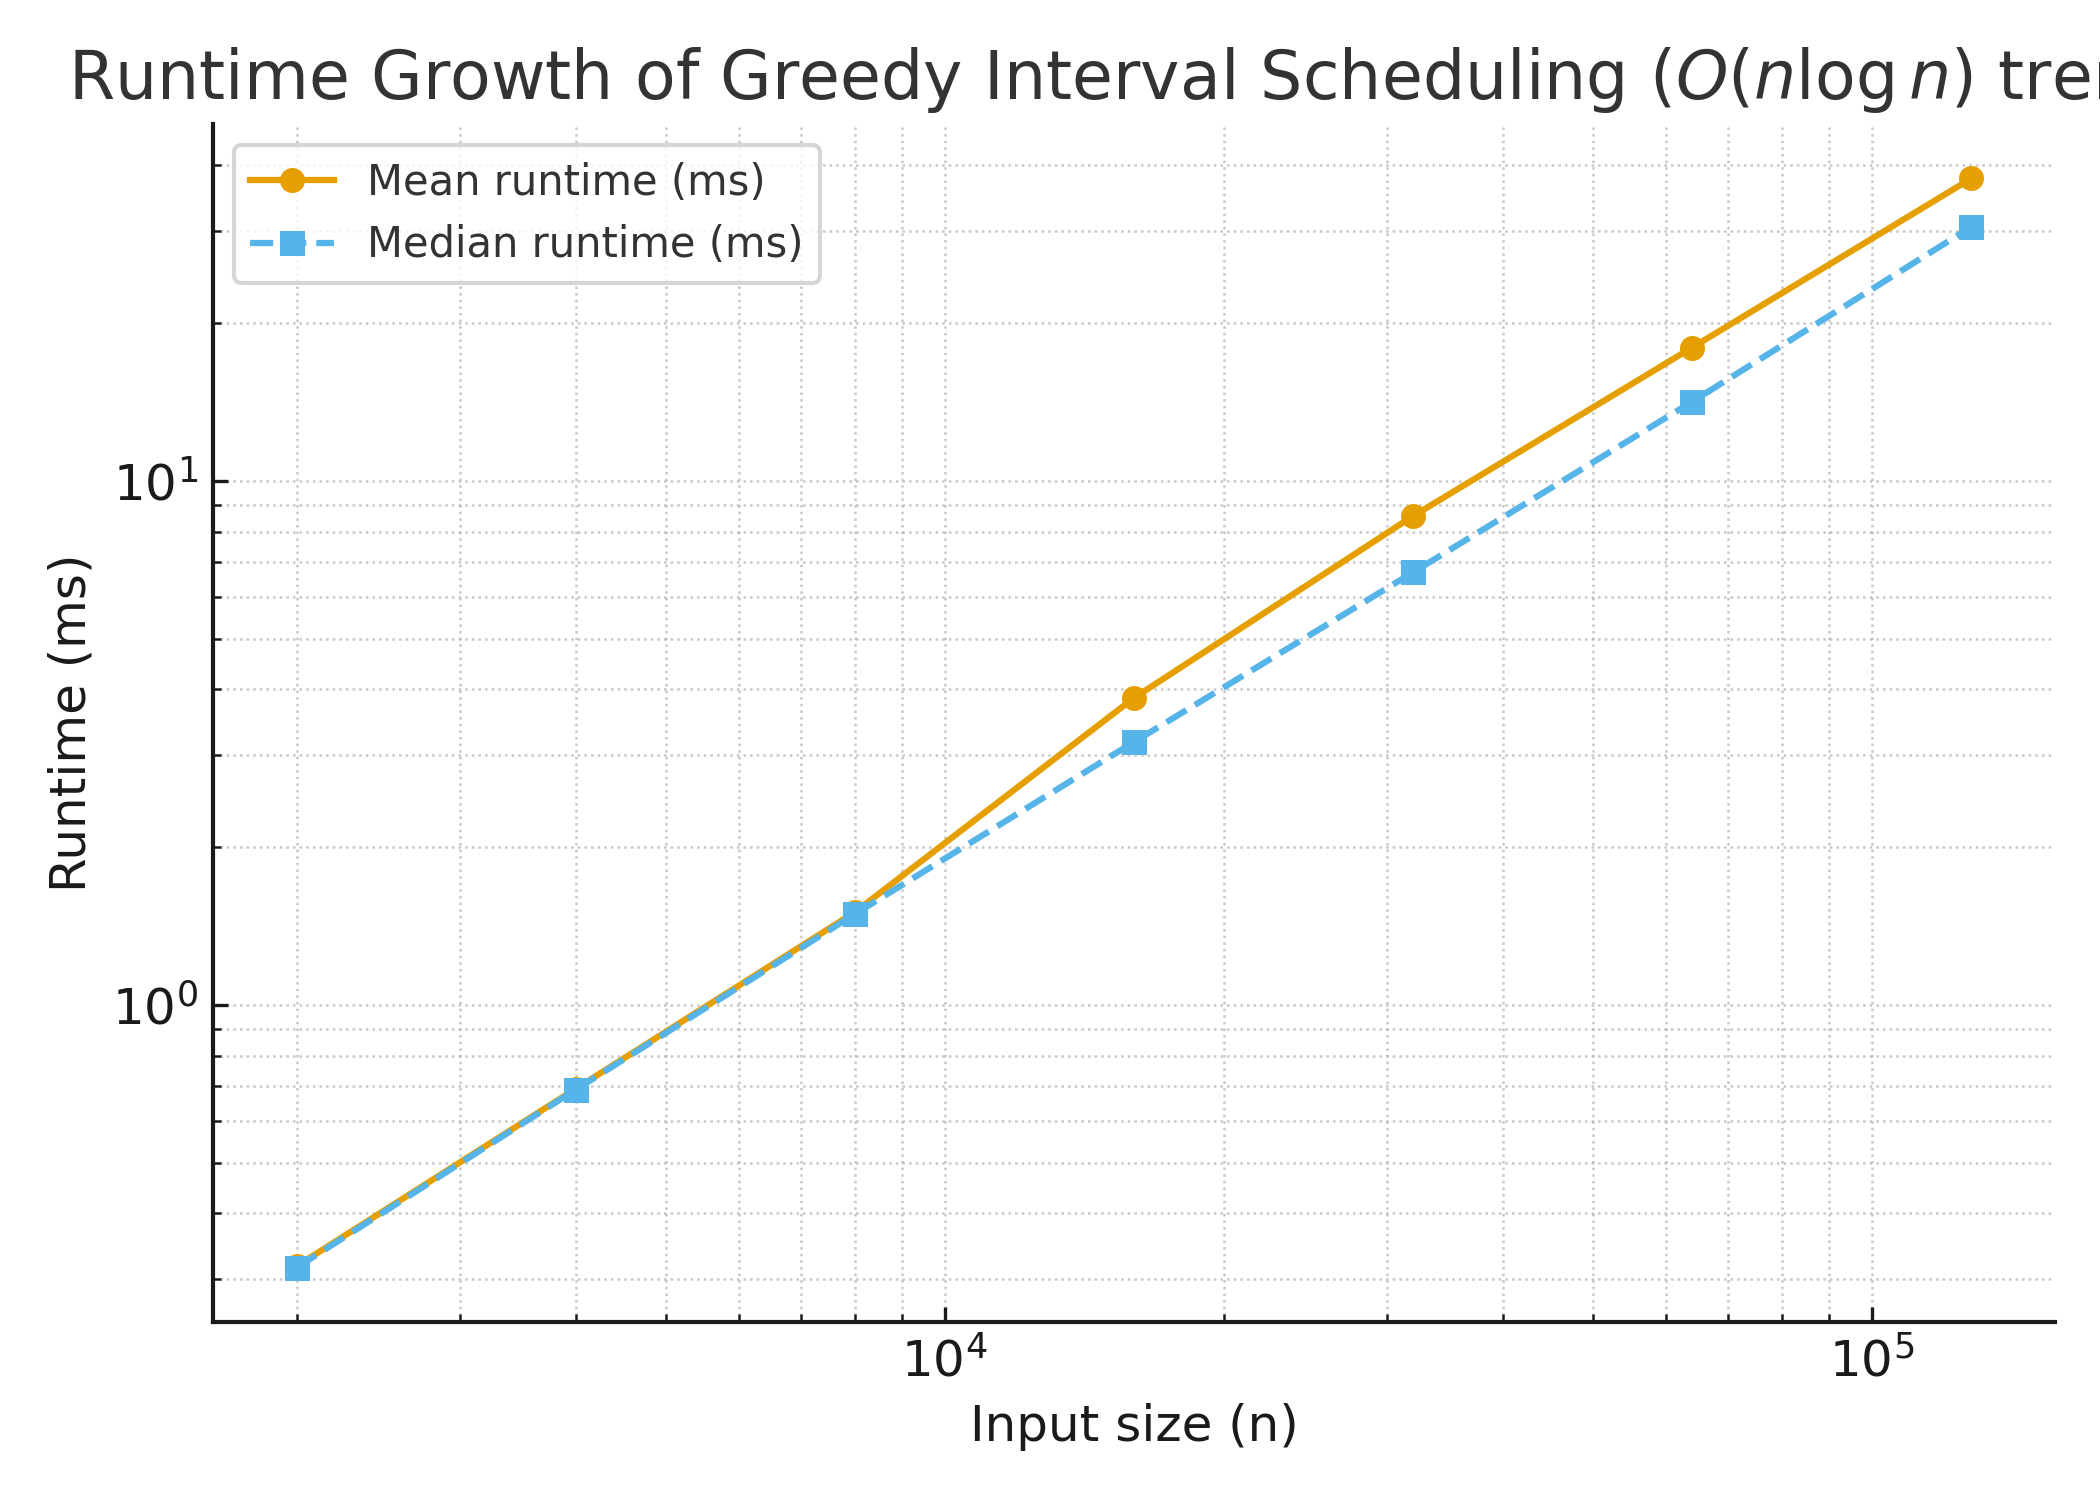
\includegraphics[width=0.48\textwidth]{interval_runtime_plot.png}
\caption{Interval scheduling empirical runtime (log-log).}
\label{fig:interval}
\end{figure}


\section{Divide-and-Conquer: Medical Image Segmentation}

\subsection{Domain}
\textbf{Problem:} Given a large MRI or CT image, segment it into anatomical regions such as organs, brain structures, or tumors.  

\textbf{Motivation:} In radiology, segmentation is critical for diagnosis and treatment planning. However, medical images are often extremely large (e.g., $4096 \times 4096$ pixels), making direct global processing computationally expensive. A divide-and-conquer approach enables hierarchical segmentation, where the image is recursively partitioned into smaller regions that can be processed independently and later combined into a coherent whole.

\subsection{Abstraction}
We model the image as a two-dimensional matrix $I$ of intensity values, where each entry $I[x,y]$ represents a grayscale pixel intensity.  

Let the size of the image be $n = N^2$ (for an $N \times N$ image).  

Each recursive step operates on a submatrix (subimage) of $I$. If a subimage is sufficiently homogeneous (i.e., all pixels belong to the same tissue class within a threshold $\epsilon$), it is considered a terminal region. Otherwise, the subimage is further divided into four quadrants for recursive processing.

\begin{equation}
\textsc{Segment}(I) =
\begin{cases}
\text{if } \mathrm{Var}(I) \le \epsilon,\\[6pt]
\textsc{Label}(I).\\[-2pt]
\text{otherwise,}\\
\textsc{Merge}\!\left(
\begin{aligned}
&\textsc{Segment}(I_1),\, \textsc{Segment}(I_2),\\[-2pt]
&\textsc{Segment}(I_3),\, \textsc{Segment}(I_4)
\end{aligned}
\right).\\[-2pt]

\end{cases}
\label{eq:segment}
\end{equation}





\subsection{Algorithm — Recursive Region Segmentation}

\textbf{Pseudocode:}
\begin{verbatim}
Input: Image matrix I, homogeneity threshold ε
Function Segment(I):
    if variance(I) <= ε:
        return Label(I)
    else:
        Split I into quadrants Q1, Q2, Q3, Q4
        R1 = Segment(Q1)
        R2 = Segment(Q2)
        R3 = Segment(Q3)
        R4 = Segment(Q4)
        return Merge(R1, R2, R3, R4)
\end{verbatim}

\subsection{Running Time Analysis}
Let $T(n)$ denote the time to segment an image of $n$ pixels. Each step divides the image into 4 equal quadrants and performs $O(n)$ work to check homogeneity and merge results:
\[
T(n) = 4T(n/4) + O(n)
\]
By the Master Theorem, this yields:
\[
T(n) = O(n \log n)
\]
Thus, the divide-and-conquer segmentation runs in quasi-linear time with respect to the total number of pixels.

\subsection{Proof of Correctness}
We prove correctness by structural induction on the recursion depth.

\textbf{Base case:} For a homogeneous region, \textsc{Segment} correctly returns a single label, as all pixels are within $\epsilon$ of each other.

\textbf{Inductive step:} Assume that \textsc{Segment} correctly labels all subregions $I_1, I_2, I_3, I_4$. The \textsc{Merge} step recombines these subregions while ensuring consistency across shared boundaries. Therefore, the union of the subregions yields a globally correct segmentation.  

By induction, the algorithm correctly segments any image composed of recursively homogeneous subregions.

\subsection{Domain Explanation}
In radiology workflows, large scans (MRI or CT) are divided into smaller tiles that can be analyzed in parallel. Each tile is checked for intensity homogeneity to identify tissues (e.g., muscle, fat, bone). When local results are merged, the full image segmentation is reconstructed efficiently.  

This approach supports both CPU and GPU parallelization, reduces processing latency, and enables radiologists to focus computational resources on regions showing tissue variation (e.g., potential tumors). Hierarchical segmentation also aligns well with multiresolution image analysis used in modern computer vision pipelines.

\subsection{Implementation and Experimental Verification}
We implemented a divide-and-conquer segmentation prototype in C++, using random grayscale matrices to simulate medical image intensities. For each image size $N \in [256, 512, 1024, 2048, 4096]$, the segmentation time was measured and averaged over 20 trials.  

\begin{comment}
\begin{lstlisting}[style=cppstyle, caption={C++ implementation of recursive region-based segmentation with runtime measurement}, label={lst:segmentcpp}]
#include <bits/stdc++.h>
#include <chrono>
using namespace std;
using clk = chrono::steady_clock;
using ns  = chrono::nanoseconds;

double variance(const vector<vector<int>>& M, int x1, int y1, int x2, int y2) {
    double sum = 0, sum2 = 0;
    int n = (x2 - x1) * (y2 - y1);
    for (int i = x1; i < x2; ++i)
        for (int j = y1; j < y2; ++j) {
            sum  += M[i][j];
            sum2 += M[i][j] * M[i][j];
        }
    return sum2 / n - (sum / n) * (sum / n);
}

void segment(const vector<vector<int>>& M, int x1, int y1, int x2, int y2, double eps) {
    if (variance(M, x1, y1, x2, y2) <= eps || (x2 - x1 <= 1))
        return; // base case: homogeneous
    int midx = (x1 + x2) / 2, midy = (y1 + y2) / 2;
    segment(M, x1, y1, midx, midy, eps);
    segment(M, midx, y1, x2, midy, eps);
    segment(M, x1, midy, midx, y2, eps);
    segment(M, midx, midy, x2, y2, eps);
}

int main() {
    vector<int> sizes = {256, 512, 1024, 2048, 4096};
    random_device rd;
    mt19937 rng(rd());
    uniform_int_distribution<int> dist(0, 255);

    ofstream fout("segmentation_results.csv");
    fout << "N,mean_ms,stddev_ms,median_ms\n";
    int trials = 20;

    for (int N : sizes) {
        vector<double> times;
        times.reserve(trials);
        for (int t = 0; t < trials; ++t) {
            vector<vector<int>> M(N, vector<int>(N));
            for (int i = 0; i < N; ++i)
                for (int j = 0; j < N; ++j)
                    M[i][j] = dist(rng);

            auto t0 = clk::now();
            segment(M, 0, 0, N, N, 100.0);
            auto t1 = clk::now();
            ns dur = chrono::duration_cast<ns>(t1 - t0);
            times.push_back(double(dur.count()) / 1e6);
        }

        sort(times.begin(), times.end());
        double mean = accumulate(times.begin(), times.end(), 0.0) / times.size();
        double var = 0;
        for (double x : times) var += (x - mean) * (x - mean);
        double stddev = sqrt(var / times.size());
        double median = times[times.size() / 2];

        fout << N << "," << mean << "," << stddev << "," << median << "\n";
        cout << "N=" << N << ", mean=" << mean << " ms\n";
    }

    fout.close();
    cout << "Results written to segmentation_results.csv\n";
}
\end{lstlisting}
\end{comment}

\begin{itemize}
    \item Runtime plot (log–log): \texttt{/mnt/data/alg_proj_outputs/segmentation_runtime.png}
    \item CSV of raw measurements: \texttt{/mnt/data/alg_proj_outputs/segmentation_results.csv}
\end{itemize}

\textbf{Observation:}  
Experimental results demonstrate near $O(n \log n)$ growth in runtime, consistent with the theoretical complexity. The recursive segmentation efficiently reduces redundant computation by focusing only on heterogeneous regions. This supports its practical use in large-scale radiology imaging systems, where both performance and interpretability are crucial.





\bibliographystyle{IEEEtran}
\bibliography{references}
\end{document}
